\documentclass[10pt,aspectratio=169,serif]{beamer}


%\setbeamertemplate{caption}[numbered]
\usefonttheme{serif}

% 中文支持：需用 XeLaTeX 编译（latexmk -xelatex main.tex）
% 中文衬线宋体：macOS 用 Songti SC；其他环境（Linux/Overleaf 等）自动回退到
% TeX Live 自带的 FandolSong（按文件名经 kpathsea 加载，不依赖系统字体）
\usepackage[fontset=none, scheme=plain]{ctex}
\IfFontExistsTF{Songti SC}{%
	\setCJKmainfont{Songti SC}[AutoFakeSlant=0.2]%
	\setCJKsansfont{Songti SC}[AutoFakeSlant=0.2]%
	\setCJKmonofont{Songti SC}%
}{%
	\setCJKmainfont{FandolSong-Regular}[Extension=.otf,BoldFont=FandolSong-Bold,AutoFakeSlant=0.2]%
	\setCJKsansfont{FandolSong-Regular}[Extension=.otf,BoldFont=FandolSong-Bold,AutoFakeSlant=0.2]%
	\setCJKmonofont{FandolFang-Regular}[Extension=.otf,BoldFont=FandolFang-Regular]%
}
\usepackage{hyperref}
\setmainfont{XCharter} % Nicer fonts — the charter package is ignored under XeLaTeX, so use fontspec instead
% 等宽字体：优先 Maple Mono NF（静态字族，真实粗/斜体），其次可变版，未安装则回退默认
\IfFontExistsTF{Maple Mono NF}{%
	\setmonofont{Maple Mono NF}[Scale=MatchLowercase,Ligatures=TeX]%
}{%
	\IfFontExistsTF{Maple Mono}{%
		\setmonofont{Maple Mono}[Scale=MatchLowercase,Ligatures=TeX]%
	}{}%
}
\usepackage{latexsym,xcolor,multicol,booktabs}
\usepackage{calligra}% 手写体英文字体
\usepackage{amsmath,amssymb,amsfonts}
\usepackage{graphicx,caption}

\usepackage{bm}
\usepackage{wrapfig}
\usepackage{ragged2e}
\usepackage{parskip}
\usepackage{tcolorbox}
\tcbuselibrary{skins}
\usepackage{XyygU}

\captionsetup[figure]{name=图,labelsep=period,aboveskip=-3pt}
\captionsetup[table]{name=表,labelsep=period}

%---------------------间距调整---------
\renewcommand{\arraystretch}{1.3}%表格行间距调整
	% 行间公式与上文/下文的垂直间距
\setlength{\abovedisplayskip}{0pt plus 2pt minus 2pt}   % 公式上方间距
\setlength{\belowdisplayskip}{10pt plus 2pt minus 2pt}   % 公式下方间距

% 短行公式（不超过行宽）的间距
\setlength{\abovedisplayshortskip}{0pt plus 2pt}
\setlength{\belowdisplayshortskip}{0pt plus 2pt}
%----------------------------------------

\usepackage{tikz}
\usepackage{pgfplots}
\usetikzlibrary{arrows.meta,positioning,calc}
\pgfplotsset{
	compat=1.18,
	every axis legend/.append style={
		at={(0.95,1)},
		anchor=north west,
		legend cell align=right,
		draw = red!75!black,
		},
	}
\title[函数的表示法]{函数的表示法（二）}
\subtitle{}
\author[好好学习，努力向上]{}
\institute{}
\date{2026-10-14}

\begin{document}

\begin{frame}
  \titlepage
\end{frame}

\section{例7：成绩分析}

\begin{frame}[t]%{例7：三名同学数学成绩分析}
\textbf{例7.} 表\ref{tab:table01}是某校高一（1）班三名同学在高一学年度六次数学测试的成绩及班级平均分表。请你对这三位同学在高一学年的数学学习情况做一个分析。

\vspace{0.5em}
\small
\begin{center}
\begin{tabular}{l|cccccc}
\toprule
\textbf{姓名} & \textbf{第1次} & \textbf{第2次} & \textbf{第3次} & \textbf{第4次} & \textbf{第5次} & \textbf{第6次} \\
\midrule
王伟 & 98 & 87 & 91 & 92 & 88 & 95 \\
张城 & 90 & 76 & 88 & 75 & 86 & 80 \\
赵磊 & 68 & 65 & 73 & 72 & 75 & 82 \\
班级平均分 & 88.2 & 78.3 & 85.4 & 80.3 & 75.7 & 82.6 \\
\bottomrule
\end{tabular}
\captionof{table}{}
\label{tab:table01}
\end{center}
\end{frame}

\begin{frame}[t]%{例7 解答}
\begin{tcolorbox}[colback=xyyg_orange!10,colframe=xyyg_orange!60,title=\textbf{解:}]
从表\ref{tab:table01}中可以知道每位同学在每次测试中的成绩，但不太容易分析每位同学的成绩变化情况。如果将每位同学的"成绩"与"测试序号"之间的函数关系分别用图象（均为6个离散的点）表示出来，那么就能直观地看到每位同学成绩变化的情况。
\end{tcolorbox}

\vspace{0.5em}

\end{frame}

\begin{frame}[t]%{例7配图：成绩变化图}
	\vspace{-1em}
\begin{center}
\begin{tikzpicture}[scale=0.85]
  \begin{axis}[
    width=14cm, height=7cm,
    axis lines=middle,
    xlabel=测试序号, ylabel=成绩,
    xmin=0.5, xmax=6.5, ymin=60, ymax=100,
    xtick={1,2,3,4,5,6},
    ytick={60,70,80,90,100},
    grid=major, grid style={gray!20},
%    legend pos= outer north east,
    ylabel style={above right},
    xlabel style={below right},
    smooth,
  ]
  % 王伟
  \addplot[very thick,magenta,dashed,mark=*,mark size=3pt] coordinates {(1,98)(2,87)(3,91)(4,92)(5,88)(6,95)};
  \addlegendentry{王伟}
  % 张城
  \addplot[very thick,blue,dashed,mark=triangle*,mark size=3pt] coordinates {(1,90)(2,76)(3,88)(4,75)(5,86)(6,80)};
  \addlegendentry{张城}
  % 赵磊
  \addplot[very thick,orange,dashed,mark=square*,mark size=3pt] coordinates {(1,68)(2,65)(3,73)(4,72)(5,75)(6,82)};
  \addlegendentry{赵磊}
  % 班级平均分
  \addplot[very thick,black,mark=o,mark size=3pt] coordinates {(1,88.2)(2,78.3)(3,85.4)(4,80.3)(5,75.7)(6,82.6)};
  \addlegendentry{班级平均分}
  \end{axis}
\end{tikzpicture}
\captionof{figure}{}
\label{fig:img-01}
\end{center}

\vspace{-10pt}
%从图\ref{fig:img-01}可以看到：
\begin{itemize}
	\item<2-> \alert{王伟}：成绩始终高于班级平均水平，学习情况比较稳定而且成绩优秀。
	\item<3-> \alert{张城}：成绩不稳定，总是在班级平均水平上下波动，而且波动幅度较大。
	\item<4-> \alert{赵磊}：成绩低于班级平均水平，但表示他成绩变化的图象呈上升趋势，表明他的数学成绩在稳步提高。
\end{itemize}
\end{frame}

\section{例8：个人所得税}

\begin{frame}[t]%{例8：个人所得税}
\vspace{-0.5em}
\textbf{例8.} 依法纳税是每个公民应尽的义务。2019年1月1日起，个税税额根据应纳税所得额、税率和速算扣除数确定：
\[
\text{个税税额} = \text{应纳税所得额} \times \text{税率} - \text{速算扣除数}. \quad \tag{1}
\]
\[
\text{应纳税所得额} = \text{综合所得收入额} - \text{基本减除费用} - \text{专项扣除} - \text{专项附加扣除} - \text{其他扣除}. \tag{2}
\]

其中，“基本减除费用”（免征额）为每年60000元。

\vspace{0.5em}
\begin{columns}
\column{0.55\textwidth}
\small

\begin{tabular}{c|c|c|c}
\toprule
级数 & 全年应纳税所得额 & 税率(\%) & 速算扣除数 \\
\midrule
1 & $[0,36000]$ & 3 & 0 \\
2 & $(36000,144000]$ & 10 & 2520 \\
3 & $(144000,300000]$ & 20 & 16920 \\
4 & $(300000,420000]$ & 25 & 31920 \\
5 & $(420000,660000]$ & 30 & 52920 \\
6 & $(660000,960000]$ & 35 & 85920 \\
7 & $(960000,+\infty)$ & 45 & 181920 \\
\bottomrule
\end{tabular}

\column{0.4\textwidth}
\small
(1) 设全年应纳税所得额为 $t$，应缴纳个税税额为 $y$，求 $y=f(t)$，并画出图象；

\addvspace{1ex}
(2) 小王全年综合所得收入额为117600元，假定缴纳的基本养老保险、基本医疗保险、失业保险等社会保险费和住房公积金占综合所得收入额的比例分别是8\%，2\%，1\%，9\%，专项附加扣除是9600元，依法确定其他扣除是560元，那么他全年应缴纳多少综合所得个税？
\end{columns}
\end{frame}

\begin{frame}[t]{例8 解答：分段函数}
\begin{tcolorbox}[colback=orange!10,colframe=orange,title=\textbf{解：(1)}]
根据表3.1-5，可得函数 $y=f(t)$ 的解析式为分段函数：
\[
y=
\begin{cases}
0.03t, & 0 \le t \le 36000, \\
0.1t - 2520, & 36000 < t \le 144000, \\
0.2t - 16920, & 144000 < t \le 300000, \\
0.25t - 31920, & 300000 < t \le 420000, \\
0.3t - 52920, & 420000 < t \le 660000, \\
0.35t - 85920, & 660000 < t \le 960000, \\
0.45t - 181920, & t > 960000.
\end{cases}\tag{3}
\]
\end{tcolorbox}
\end{frame}

\begin{frame}[t]{例8图：个税分段函数图象}
\begin{center}
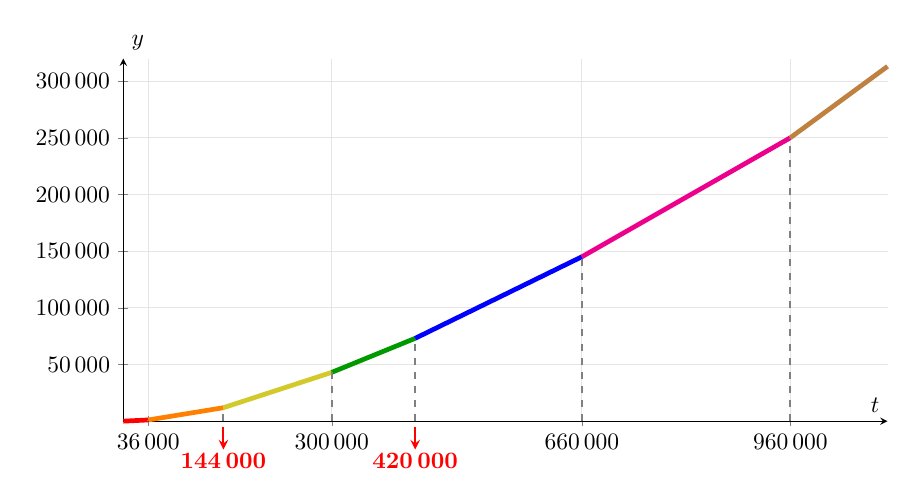
\begin{tikzpicture}[scale=0.85]
  \begin{axis}[
  	clip =false,
    width=13cm, height=7cm,
    axis lines=middle,
    xlabel=$t$, ylabel=$y$,
    xmin=0, xmax=1100000, ymin=0, ymax=320000,
    scaled ticks=false,
    xtick={0,36000,300000,660000,960000},   
    xticklabels={$O$,36\,000,300\,000,660\,000,960\,000},
%    extra x ticks={144000,420000},
%    extra x tick labels={144\,000,420\,000},
    ytick={0,50000,100000,150000,200000,250000,300000},    
    extra tick style={
    	tick label style={blue,font=\bfseries,yshift=-1em},
    },
    yticklabels={$O$,50\,000,100\,000,150\,000,200\,000,250\,000,300\,000},
    grid=major, grid style={gray!20},
    ylabel style={above right},
  ]
  % 第1段 0-36000: y=0.03t
  \addplot[line width=2pt,red,domain=0:36000,samples=2] {0.03*x} ;
  % 第2段 36000-144000: y=0.1t-2520
  \addplot[line width=2pt,orange,domain=36000:144000,samples=2] {0.1*x-2520};
  % 第3段 144000-300000: y=0.2t-16920
  \addplot[line width=2pt,yellow!80!black,domain=144000:300000,samples=2] {0.2*x-16920};
  % 第4段 300000-420000: y=0.25t-31920
  \addplot[line width=2pt,green!60!black,domain=300000:420000,samples=2] {0.25*x-31920};
  % 第5段 420000-660000: y=0.3t-52920
  \addplot[line width=2pt,blue,domain=420000:660000,samples=2] {0.3*x-52920};
  % 第6段 660000-960000: y=0.35t-85920
  \addplot[line width=2pt,magenta,domain=660000:960000,samples=2] {0.35*x-85920};
  % 第7段 >960000: y=0.45t-181920
  \addplot[line width=2pt,brown,domain=960000:1100000,samples=2] {0.45*x-181920};

  % 分段点垂直虚线
  \addplot[dashed,gray,thick,mark=none] coordinates {(36000,0)(36000,1080)};
  \addplot[dashed,gray,thick,mark=none] coordinates {(144000,0)(144000,11880)};
  \addplot[dashed,gray,thick,mark=none] coordinates {(300000,0)(300000,43080)};
  \addplot[dashed,gray,thick,mark=none] coordinates {(420000,0)(420000,73080)};
  \addplot[dashed,gray,thick,mark=none] coordinates {(660000,0)(660000,145080)};
  \addplot[dashed,gray,thick,mark=none] coordinates {(960000,0)(960000,250080)};
	\node[below=10pt,red,font=\bfseries] at (axis cs:144000,0) {144\,000};
	\draw[-stealth,red,thick] (axis cs:144000,-5000) -- (axis cs:144000,-25000);
	
	\node[below=10pt,red,font=\bfseries] at (axis cs:420000,0) {420\,000};
	\draw[-stealth,red,thick] (axis cs:420000,-5000) -- (axis cs:420000,-25000);
  \end{axis}
  
\end{tikzpicture}
\captionof{figure}{}
\label{fig:img02}
\end{center}
\end{frame}

\begin{frame}[t]{例8 解答：小王个税计算}
\begin{tcolorbox}[colback=orange!10,colframe=orange,title=\textbf{解：(2)}]
根据公式(2)，小王全年应纳税所得额为：
\[
\begin{aligned}
t &= 117600 - 60000 - 117600 \times (8\% + 2\% + 1\% + 9\%) - 9600 - 560 \\
&= 0.8 \times 117600 - 70160 \\
&= 23920.
\end{aligned}
\]

将 $t$ 的值代入（3），得：
\[
y = 0.03 \times 23920 = 717.6.
\]

所以，小王应缴纳的综合所得个税税额为 \alert{717.6元}。
\end{tcolorbox}
\end{frame}

\section{练习}

\begin{frame}[t]{练习1：图象与事件匹配}
\textbf{练习1.} 下图中哪几个图象与下述三件事分别吻合得最好？请你为剩下的那个图象写出一件事。

\begin{enumerate}
  \item 我离开家不久，发现自己把作业本忘在家里了，于是返回家里找到了作业本再上学；
  \item 我骑着车离开家后一路匀速行驶，只是在途中遇到一次交通堵塞，耽搁了一些时间；
  \item 我从家出发后，心情轻松，一路缓缓加速行进。
\end{enumerate}
\begin{center}
	\begin{tikzpicture}[scale=0.7,>=stealth]
		% 图A
		\begin{scope}[shift={(0,0)}]
			\draw[->,thick] (0,0) -- (3,0) node[below]{时间};
			\draw[->,thick] (0,0) -- (0,3) node[above,anchor=west]{离开家的距离};
			\draw[magenta,thick] (0,0) -- (0.8,1) -- (1.8,1) -- (2.8,2.2);
			\node[below] at (1.5,-0.5) {(A)};
		\end{scope}
		% 图B
		\begin{scope}[shift={(4,0)}]
			\draw[->,thick] (0,0) -- (3,0) node[below]{时间};
			\draw[->,thick] (0,0) -- (0,3) node[above,anchor=west]{离开家的距离};
			\draw[magenta,thick] plot[domain=0:2.5,samples=50] (\x,{0.3*\x*\x});
			\node[below] at (1.5,-0.5) {(B)};
		\end{scope}
		% 图C
		\begin{scope}[shift={(8,0)}]
			\draw[->,thick] (0,0) -- (3,0) node[below]{时间};
			\draw[->,thick] (0,0) -- (0,3) node[above,anchor=west]{离开家的距离};
			\draw[magenta,thick] plot[domain=0:2.5,samples=50] (\x,{1*sqrt(\x)});
			\node[below] at (1.5,-0.5) {(C)};
		\end{scope}
		% 图D
		\begin{scope}[shift={(12,0)}]
			\draw[->,thick] (0,0) -- (3,0) node[below]{时间};
			\draw[->,thick] (0,0) -- (0,3) node[above,anchor=west]{离开家的距离};
			\draw[magenta,thick] (0,0) -- (0.7,1.2) --(0.9,1.2) -- (1.5,0) -- (2.2,0) -- (2.8,2);
			\node[below] at (1.5,-0.5) {(D)};
		\end{scope}
	\end{tikzpicture}
\end{center}
\end{frame}



\begin{frame}[t]{练习1 解答}
\begin{tcolorbox}[colback=orange!10,colframe=orange,title=\textbf{解:}]
\begin{itemize}
  \item 事件(1) 与图\alert{D} 吻合：离开家→返回家（距离为0）→再出发上学。
  \item 事件(2) 与图\alert{A} 吻合：匀速行驶→堵塞（距离不变）→继续行驶。
  \item 事件(3) 与图\alert{C} 吻合：缓缓加速（斜率逐渐增大，曲线向上凸）。
\end{itemize}

\vspace{0.5em}
剩下的图\alert{B}：可以描述"我从家出发后，一路加速行驶，速度越来越快"或"我爬山时，海拔高度随时间越来越快地上升"等。
\end{tcolorbox}
\end{frame}

\begin{frame}[t]{练习2：公共汽车票价}
\textbf{练习2.} 某市"招手即停"公共汽车的票价按下列规则制定：

\begin{enumerate}
  \item 5 km以内（含5 km），票价2元；
  \item 5 km以上，每增加5 km，票价增加1元（不足5 km的按5 km计算）。
\end{enumerate}

如果某条线路的总里程为20 km，请根据题意，写出票价与里程之间的函数解析式，并画出函数的图象。
\end{frame}

\begin{frame}[t]{练习2 解答}
\begin{tcolorbox}[colback=orange!10,colframe=orange,title=\textbf{解:}]
设里程为 $x$ km，票价为 $y$ 元。根据题意：

\[
y =
\begin{cases}
2, & 0 < x \le 5, \\
3, & 5 < x \le 10, \\
4, & 10 < x \le 15, \\
5, & 15 < x \le 20.
\end{cases}
\]

这是一个分段函数（阶梯函数），定义域为 $(0, 20]$，值域为 $\{2, 3, 4, 5\}$。
\end{tcolorbox}
\end{frame}

\begin{frame}[t]{练习2配图：票价阶梯图}
\begin{center}
\begin{tikzpicture}[scale=0.9]
  \begin{axis}[
    width=12cm, height=7cm,
    axis lines=middle,
    xlabel=里程(km), ylabel=票价(元),
    xmin=0, xmax=22, ymin=0, ymax=6,
    xtick={0,5,10,15,20},
    ytick={2,3,4,5},
    grid=major, grid style={gray!20},
    xlabel style={above},
    ylabel style={right},
  ]
  % 阶梯函数：开区间在左，闭区间在右
  \addplot[very thick,blue] coordinates {(0,2) (5,2)};
  \addplot[very thick,blue] coordinates {(5,3) (10,3)};
  \addplot[very thick,blue] coordinates {(10,4) (15,4)};
  \addplot[very thick,blue] coordinates {(15,5) (20,5)};
  % 端点
  \addplot[only marks,mark=*,mark size=3pt] coordinates {(5,2)(10,3)(15,4)(20,5)};
  \addplot[only marks,mark=*,mark size=3pt,mark options={fill=white}] coordinates {(0,2)(5,3)(10,4)(15,5)};
  \end{axis}
\end{tikzpicture}
\end{center}
\end{frame}

\begin{frame}[t]{布置作业}
	课本 P73： 8---12
\end{frame}

\begin{frame}[c]
%  \begin{center}
%    {\Huge 谢谢！}
%  \end{center}
    \begin{center}
	{\Huge\calligra Thanks!}
\end{center}
\end{frame}

\end{document}
